% Results
% This section may be divided by subheadings. Footnotes should not be used and must be transferred to the main text.

\section{Results and Discussion}

Here we detail the results of all experiments and place them in the broader landscape of historical contingency literature. 

\begin{figure}[h!]
\begin{center}
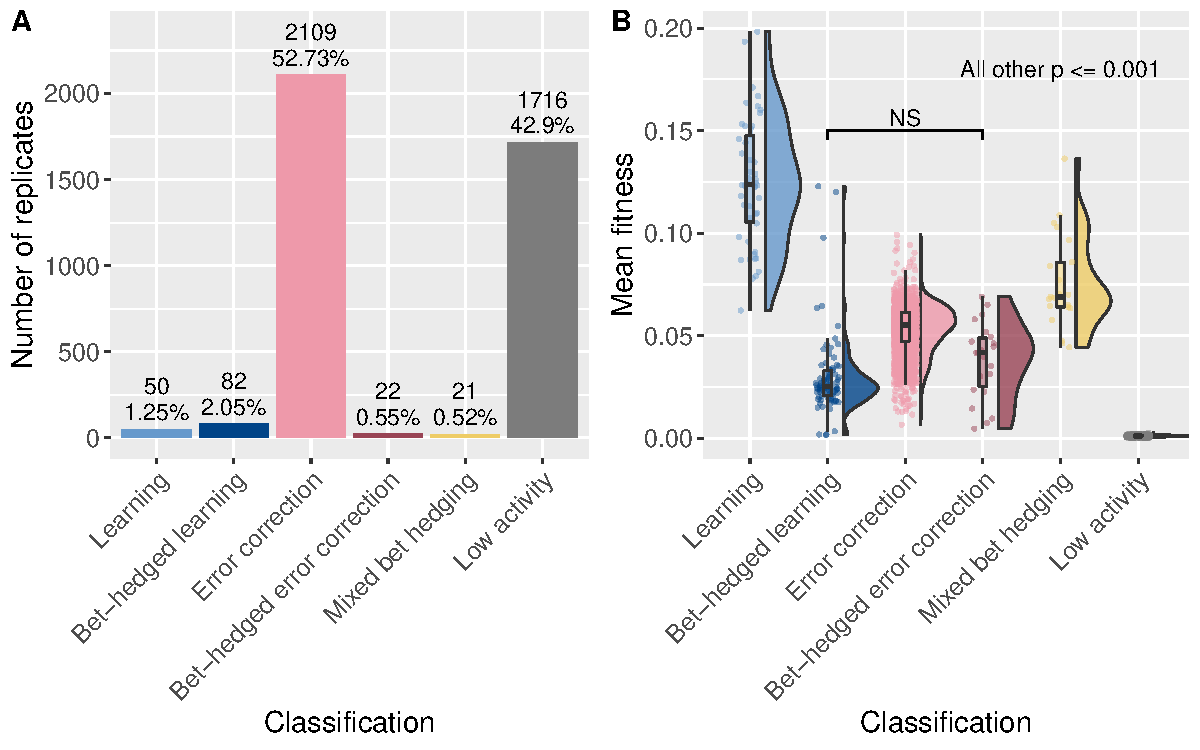
\includegraphics[width=0.9\textwidth]{04_learning_extension/media/initial_reps_stats.pdf}
\end{center}
\caption{ 
Subplot A) Columns show the number of initial replicates whose representative genotype evolved each type of behavior. 
Above each column, the numbers show the number of replicates that evolved that behavior and that count as a percentage of all 4,000 replicates. % (out of 4,000), while the bottom number shows the fraction of replicates.
Subplot B) Raincloud plots show fitness of all 4,000 initial replicates' representative genotypes, grouped by evolved behavior.
All pairwise comparisons are highly significant (p <= 0.001; Pairwise Mann-Whitney with Bonferroni correction) except for the one marked pair (bet-hedged learning and bet-hedged error correction did not have a significant difference).
}\label{fig:initial_reps}
\end{figure}


\subsection{The evolution of learning is exceedingly rare on random paths}
% Initial replicates (Outline)
    % Show categorical outcome figure
    % Learning DOES evolve, but only 1.25% of the time
    % Low activity and error correction account for >95% of replicates
    % Everything else is rare <= 3%
    % We can also look at fitness
        % We see that learning is the most efficient behavior
            % There is some overlap with learning-adjacent behavior (bet-hedged learning / mixed strategy bet-hedging)
        % Otherwise, error correction isn't too far behind learning (sig?)
    % Why is learning so rare here? 
            % It evolved in 8% of replicates in the other chapter
            % And even more than that in Anselmo's work
            % But here, we are evolving on *purely random paths*
            % This removes the first-cue guarantees, and creates a much more challenging bootstrapping problem

As shown in Figure \ref{fig:initial_reps}A, associative learning evolved in only 50 of 4,000 replicates (1.25\%). 
This is considerably lower than the probability of evolving associative learning in previous work, with 8\% of replicates evolving learning in Chapter \ref{chap:learning_case_studies} and up to 14\% in the ``two fixed turns'' environment of \citep{pontesEvolutionaryOriginAssociative2020}.
However, these higher success rates where observed in environments that guaranteed the order of one or more turns at the start of each path. 
In this work we have removed those guarantees entirely; the next step in the path is always uniformly chosen at random among a left turn, right turn, or a step straight ahead.
Thus, we must compare these results to the ``random start'' experiments in 
\citep{pontesEvolutionaryOriginAssociative2020}. 
In their work, zero of 50 replicates evolved learning under such conditions. 
This work therefore marks the first time that associative learning has evolved in Avida without any guarantees about cue ordering. 
It should be mentioned, however, that this work is more lenient with the \texttt{Move Backward} instruction, placing the organism directly back on the path instead of moving them one tile backward and requiring them to reorient on their own, as in \citep{pontesEvolutionaryOriginAssociative2020}.

While learning rarely evolved, error correcting behaviors evolved in the majority (53\%) of replicates. 
Similarly, most of the other replicates (43\%) were classified as ``Low Activity'' as, even at the end of the evolutionary replicate, they failed to correctly identify at least 25 cues in any of 100 trials. 
The remaining replicates evolved bet-hedged behaviors, with bet-hedged learning, bet-hedged error correction, and mixed bet hedging each present in less than 3\% of final evolved populations.

Finally, we see that organisms that perform learning have significantly higher fitness than organisms performing any other strategy (Figure \ref{fig:initial_reps}B, all $p << 0.001$, pairwise Mann Whitney with Bonferroni corrections for multiple comparisons). 
Mixed bet hedging has the next highest fitness, falling between its two constituent parts, learning and error correction. 
Bet-hedged learning and bet-hedged error correction both have lower fitness, on average, than their non-bet hedged counterparts. 
Finally, ``Low activity'' has very low fitness, as expected. 
These fitness values show us that learning was not rare because it was a poor solution to the problem, but rather due to the rugged nature of the underlying fitness landscape.

%\subsection{All replicates see windows of significant potentiation gain}
\subsection{Substantial increases in potentiation are common}

% Substantial increases in potentiation are common
    % We can look at this at two levels: 
        % 1. Exploratory (windows)
        % 2. Targeted (individual steps)
    % At the exploratory level *every* replayed replicate shows significant increase within a single window
        % This varies quite a bit, as we see in the distribution figures
    % At the targeted level, most replayed replicates show significant increase with a single step
        % But not all, we have exactly one non-significant replicate, and a few more are only weakly significant (p <= 0.05)
    % Is this consistent with preexisting replay replicates? 
        % In our work, yes!
        % Other digital studies?
            % Yedid? 
            % Covert?
        % In natural systems...
            % Zach's work... maybe?
            % Meyer paper?
            % C Turner paper? 
            % Jochmusen?
            % Other new papers?

\begin{figure}[h!]
\begin{center}
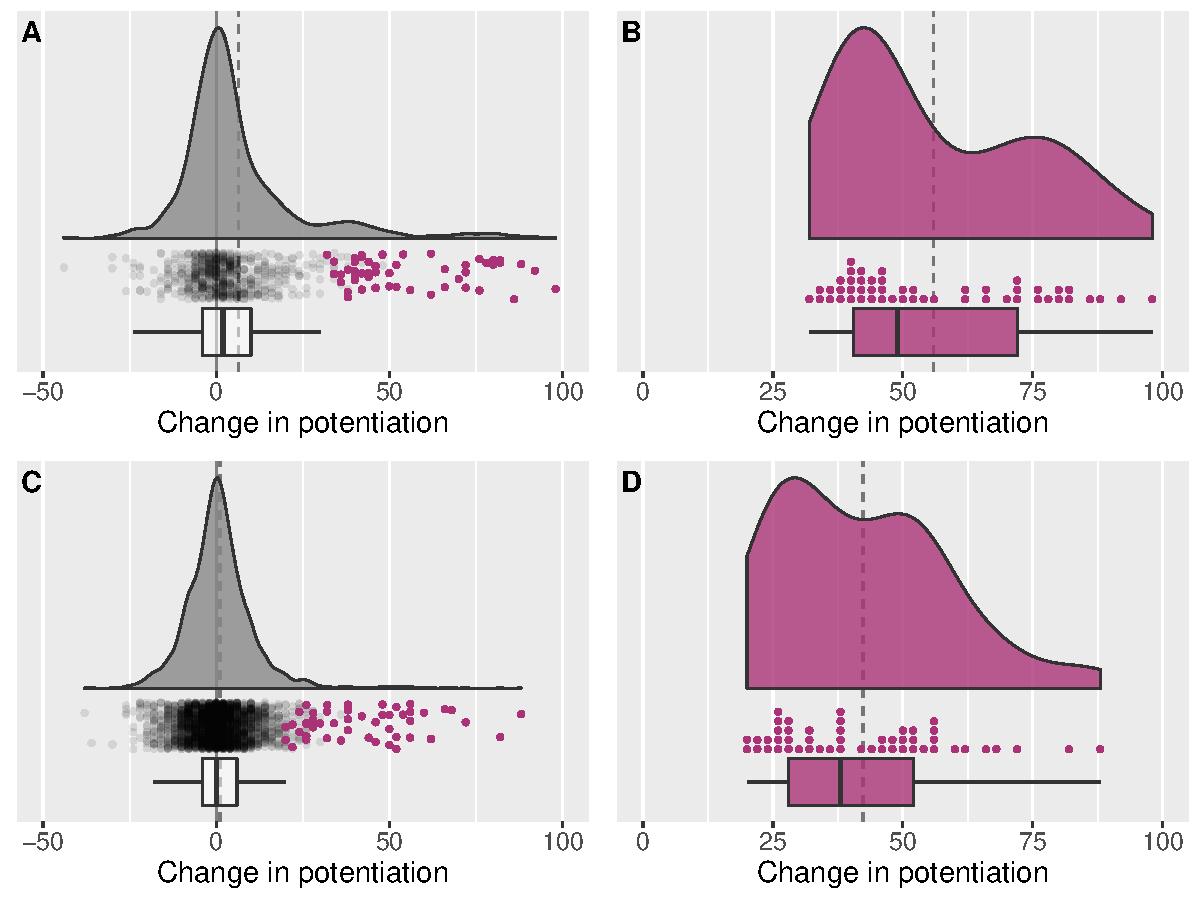
\includegraphics[width=0.9\textwidth]{04_learning_extension/media/replays_dists.pdf}
\end{center}
\caption{ 
Aggregate data for the exploratory replays (A,B) and targeted replays (C,D) of learning replicates. 
Subplots A and C) Raincloud plots showing the distribution of potentiation changes for the cumulative effects across all replayed windows (A) or the individual effects of all replayed lineage steps (C).
The solid vertical line shows zero change and the dashed vertical line shows the mean of the potentiation changes. 
For each of the 50 replicates, a purple point shows the maximum single-window (A) or single-step (C) potentiation increase.
These 50 points are then shown in isolation in (B) and (D).
Subplots B and D)  Raincloud plots showing the distribution of maximum single-window (B) or single-step (D) potentiation changes for each replicate (one point for each of the 50 learning replicates). 
The dashed vertical line shows the mean of these changes. 
}\label{fig:replay_distributions}
\end{figure}

\begin{figure}[h!]
\begin{center}
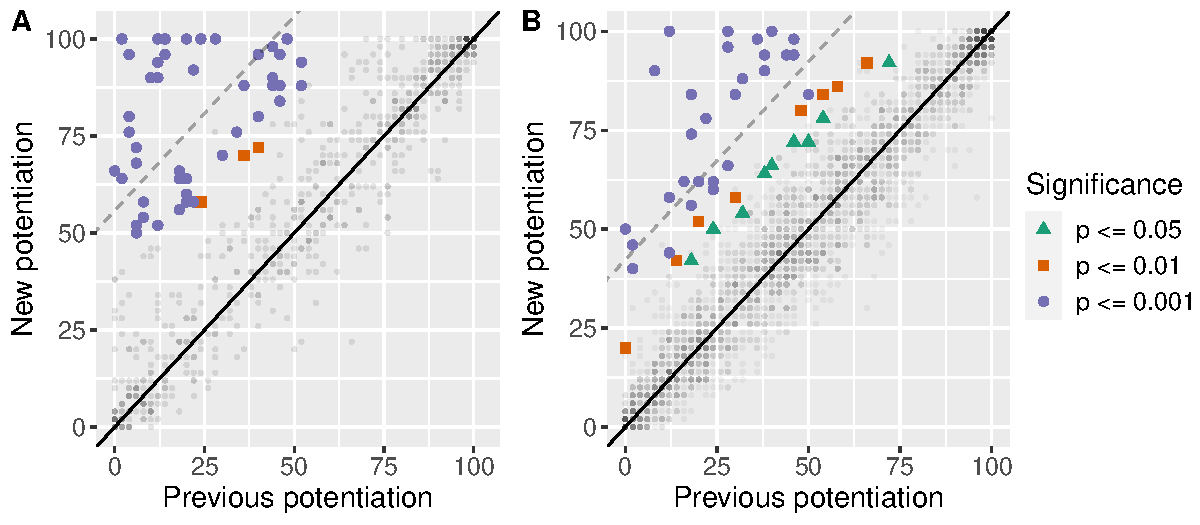
\includegraphics[width=0.9\textwidth]{04_learning_extension/media/replays_stats_legend_on_right.pdf}
\end{center}
\caption{ 
Scatter plot showing the potentiation before and after each exploratory window (Subplot A) or lineage step (Subplot B). 
The color and shape of the 50 main points show significance of the potentiation change (Fisher's exact test).
Semi-transparent points show the rest of the per-window (A, 10\% opacity) or per-step (B, 5\% opacity) potentiation changes. 
The line shows $y=x$, or no potentiation change. 
Potentiation gain is the vertical distance to this line. 
The dashed line shows the maximum potentiation gain of each replicate, averaged across all 50 replicates. 
}\label{fig:replay_stats}
\end{figure}

\begin{figure}[h!]
\begin{center}
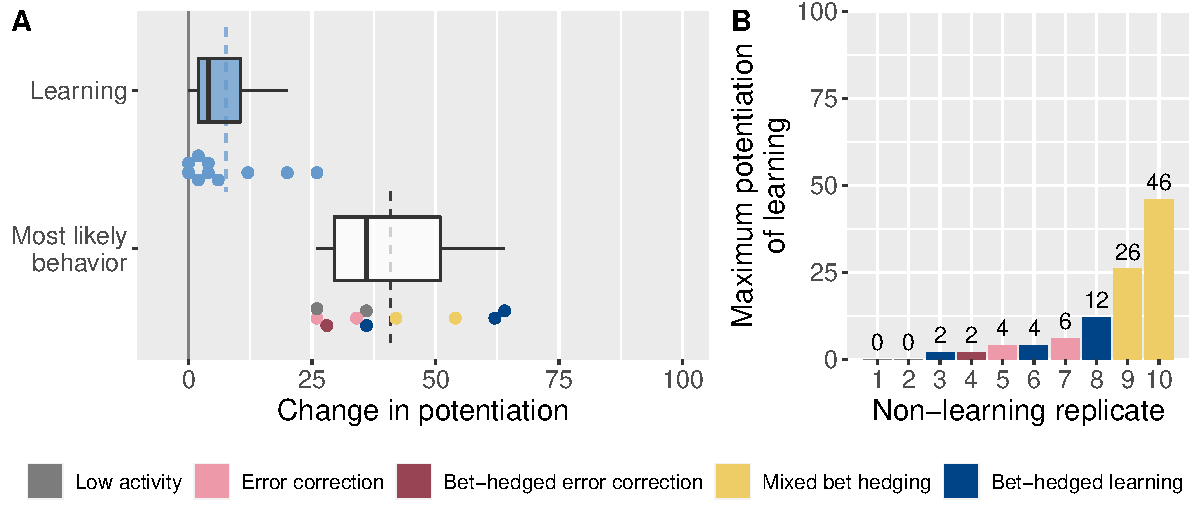
\includegraphics[width=0.9\textwidth]{04_learning_extension/media/non_learning_with_max.pdf}
\end{center}
\caption{ 
Subplot A) Distribution of the maximum per-window change in potentiation for learning (top) and most likely behavior to evolve (bottom) of each of the 10 replayed non-learning replicates.
Colors for the bottom distribution indicate the most likely behavior for each replicate.
Vertical dashed lines show the mean for each group.
Subplot B) The maximum potentiation level of learning observed in each of the 10 non-learning replicates, sorted. 
}\label{fig:non_learning}
\end{figure}

By number of replays conducted, this work is the largest study of potentiation via analytic replay experiments to date. 
Here we detail the key finding of this work: large increases in potentiation are not only possible, but are \textit{common} in this system.
This result is supported at multiple levels, as we detail below. 
For all 50 replicates, figures showing potentiation over time for both exploratory and targeted replays are available in the \hyperref[chap:app_a]{appendix}.

\subsubsection{All replicates have windows of significant potentiation gain}

Exploratory replays show us that, on average, the 50-step windows we replay show little potentiation gain (mean $\approx 6$, median = 2 percentage points) (see Figure \ref{fig:replay_distributions}A).
However, we see that these replays also cover a wide range, from -44 (i.e., 44 percentage points of potentiation \textit{loss)} to $+98$ (i.e., effectively full gain in potentiation in only 50 lineage steps). 

%When we consider the 50 learning replicates, we can also examine the maximum potentiation gain of each replicate (i.e., the potentiation gain of the \textit{potentiating window}).
When we consider these 50 learning replicates, we can also examine the maximum per-window potentiation gain of each replicate.
These maximum gains are highlighted in Figure \ref{fig:replay_distributions}A and shown in isolation in Figure \ref{fig:replay_distributions}B.
When only considering these maximum per-replicate gains, we see a mean gain of approximately $+56$, a median gain of $+49$, and a range of $[+32, +98]$ percentage points.
Figure \ref{fig:replay_stats}A shows all potentiation gains as a combination of their previous and new potentiation values. 
We see that potentiation increases significantly for all 50 learning replicates, even with only 50 replays each ($p \leq 0.01$, Fisher's exact). 
Indeed, 47 of these replicates are highly significant ($p \leq 0.001$). 
Thus we have further evidence that potentiation of learning can increase considerably in a relatively short amount of time. 

%\subsection{Large jumps in potentiation exist in most, but not all, replicates}
% \subsubsection{Large single-step increases in potentiation exist in most, but not all, replicates}
\subsubsection{Significant single-step increases in potentiation exist in all replicates}

While we see these large increases in potentiation over 50-step intervals, we can also look at smaller timescales. 
Indeed, the targeted, single-step replay results tell a similar story. 
Figure \ref{fig:replay_distributions}D shows the potentiation gains at \textit{all} replayed steps.
Here, the mean is approximately $+1$, the median is 0, and the range is $[-38, +88]$ percentage points. 
Thus we see a similar trend to the exploratory replays: the bulk of the distribution residing near zero, but with a short tail in the negative direction and a long tail in the positive direction. 

Focusing on only the maximum potentiating step for each lineage (Figure \ref{fig:replay_distributions}D), we see a mean of approximately $+42$, a median of $+38$, and a range of $[+20, +88]$ percentage points. 
Immediately we see that, in many replicates, a single step in the dominant lineage can account for 50 percentage points of the potentiation of associative learning. 
However, not all replicates see these huge jumps; multiple replicates have a potentiating step of less than 25 percentage points. 
When we examine the individual potentiating steps (Figure \ref{fig:replay_stats}B), we see that all of these changes are significant. 
Of the 50 replicates, 32 were significant at $p \leq 0.001$, nine more at $p \leq 0.01$, and the final nine additional replicates at $p \leq 0.05$. 

\subsubsection{Non-learning replicates see windows of potentiation increase in other behaviors}

We also see evidence of large gains in potentiation of behaviors other than learning. 
Figure \ref{fig:non_learning} details the results of our ten non-learning replicates that were replayed. 
Of these 10 replicates, the single-window potentiation gains for learning were relatively small, with a mean increase of $+7.6$, median of $+4$, and a range of $[0, +26]$ percentage points.
These low values are not surprising, however, as these lineages did not ultimately evolve learning. 
The potentiation for learning was never actualized and eventually lost. 
It should be noted that, even so, a potentiation gain of 26 percentage points over 50 lineage steps is substantial, which is highly significant ($p \leq 0.001$, Fisher's exact). 
Indeed, we see that one of the ten replicates reached a maximum learning potentiation of 46\% at one point in its evolutionary history, though seven replicates never crossed more than a 6\% chance of evolving learning (Figure \ref{fig:non_learning}B).

While the non-learning replicates did not see large increases in the potentiation of learning, they did see large increases in the potentiation of other behaviors. 
Figure \ref{fig:non_learning}A also shows the largest per-window potentiation increase in the most likely behavior at the end of evolution. 
Here we see a mean of $+40.8$, a median of $+36$, and a range of $[+26, +64]$ percentage points.
All of these differences are significant ($p \leq 0.01$, Fisher's exact), and eight of them highly significant ($p \leq 0.001$). 
Thus, the large increases in potentiation that we have observed are \textit{not} limited to the evolution of learning. 
% It should also be noted that two behaviors, error correction and low activity, are limited in their maximum potentiation gain. 
% Since both behaviors have a $>40\%$ chance of evolving from the naive ancestor (Figure \ref{fig:initial_reps}A), they either must first decrease in potentiation, or they are capped at $<60$ percentage points of gain in potentiation, and thus it is unlikely we would witness a 80 percentage point increase like we observed in the some learning replicates. 
Our expectation is that we would observe large single-step potentiation increases for these non-learning behaviors too if we conducted targeted replays on these lineages.
Figures of how potentiation changed over time for all 10 non-learning replicates are available in the \hyperref[chap:app_a]{appendix}. 
%appendix \ref{chap:app_a} (Figure \ref{fig:app_a_non_learning}).

\subsubsection{Comparison to other works}

In addition to a deeper investigation into the underlying patterN associated with historical contingency, the original motivation for this work was to validate the findings of Chapter \ref{chap:learning_case_studies} and provide evidence as to their generality. 
That is, we wanted to test if the large per-window and per-step increases we observed in that work were common or if they were mere flukes. 
Indeed, we can now confirm that both the per-window and single-step potentiation increases from that chapter are common in this particular system. 
The maximum per-step potentiation increases we observed in the previous chapter (range of $[+36, +64]$ percentage points) fall comfortably within the range that we observe here ($[+20, +88]$ percentage points).

% Our one direct comparison -- Blount et al. 2008
% Their jumps were much smaller
It is more difficult to compare these results to other works, however. 
While several works have leveraged replay experiments to study the potentiation of a particular trait or behavior, only one has applied replays to multiple points in a single lineage \citep{blountHistoricalContingencyEvolution2008}.
Blount et al. replayed multiple time points of frozen \textit{E. coli} from the Ara-3 strain to empirically test the potentiation of citrate metabolism. 
The largest jump in potentiation they found was \localapprox $+13.3\%$, shifting from $0/30$ replicates at generation 31,500 to $4/30$ replicates at generation 32,000 %(i.e., \localapprox 13.3 percentage points across 500 generations). 
This is a much smaller jump in potentiation, measured over a much longer period of time compared to our results in this work as the tests were 500 generations apart.

% Why might we be seeing larger increases in potentiation than in natural systems?
% There are a few (possibly confounding) factors:
% 1) The genetic landscape is much less complicated here than in natural organisms. 
% While Avida is much more complicated than many digital evolution systems, and in this particular system we have the possibility for many mutations from any given genotype (e.g., $>9000$ possible one-step mutations from a genome of length 100), this is nearly trivial in comparison to natural organisms. 
% This could mean that while there are many possible evolutionary paths in this system, there are still significantly fewer possibilities than in natural systems, and thus any individual paths is at a higher probability of selection. 
% 2) A lack of behavior-refinement needed in this system -- as discussed in \citep{blountGenomicAnalysisKey2012}, citrate metabolism underwent considerable refinement after it first evolved, and thus mutations to citrate metabolism might be lost to drift more frequently than learning-actualizing mutations in this system. 
% While associative learning in this system can be refined, we use an ``all or nothing'' definition and thus anything classified as learning should be relatively fit. 
% 3) E.coli evolved well over 100 million years ago, which should imply that they have settled into a rather stable region of the fitness landscape...


% The other good comparison -- Jochmusen et al 2016
While not directly pulling from an evolving lineage, \citet{jochumsenEvolutionAntimicrobialPeptide2016a} tested the effects of individual mutations on the evolution of colistin resistance in \textit{Pseudomonas aeruginosa}. 
Via experimental evolution, they found evidence that two individual mutations (\textit{phoQ} and \textit{pmrB}) each potentiated the evolution of colistin resistance at the $16\frac{\mu g}{ml}$ concentration level.
These two mutations each increased the potential to evolve this colistin level from  a $<5\%$ chance to a $>70\%$ chance. 
These results directly align with our results -- that a single mutation can drastically increase the probability of a focal behavior evolving. 

% Other works
% Caroline's work -- Never saw extinction in a replay
% Justin Meyer's work -- They were comparing across strains
% Art Covert's work -- Strong effect of a single deleterious mutation
% Dave Bryson's dissertation -- Strong effects in short term replays
For other works, \citet{turnerReplayingEvolutionTest2015} performed similar analytic replay techniques, but never saw the focal results -- the extinction of the Cit$^{-}$ clade in the Long Term Evolution Experiment -- in any of the replay replicates. 
\citet{meyerRepeatabilityContingencyEvolution2012} replayed combinations of Phage $\lambda$ and \textit{E. coli}. 
While some of their results are striking (e.g., the ``all-or-nothing`` pattern of OmpF receptor targeting across certain treatments), the comparisons were across strains and thus not a direct comparison. 
In prior digital work, \citet{covertiiiExperimentsRoleDeleterious2013} showed that a single deleterious mutation could increase the evolution of a complex behavior in Avida (the EQU logic task) from 13/20 (65\%) to 20/20 (100\%) of evolutionary replicates, providing further evidence of substantial potentiation gain from a single mutation.
Similarly, \citet{brysonEvolutionaryPotentialPopulations2012} showed multiple instances of $\geq 50$ percentage points of increase in short-term (always 10,000 updates) replays of EQU in Avida. 

% Do we want a paragraph summarizing these different results? 
% Most studies you cannot compare
% Those you can are mixed
%   A few have small changes (Blound, Turner)
%   Others match well (Jochmusen, Meyer, Covert III, Bryson)

\subsection{Increases in potentiation are often driven by a single mutation}
% Single mutations often drive increases in potentiation
    % Of our 50 replayed learning replicates, the largest potentiation step occured with only one mutation in 30 replicates
    % Of the 30 other replicates, we see that 14 of them have exactly one significant contributor, which is a standalone mutation

\begin{figure}[h!]
\begin{center}
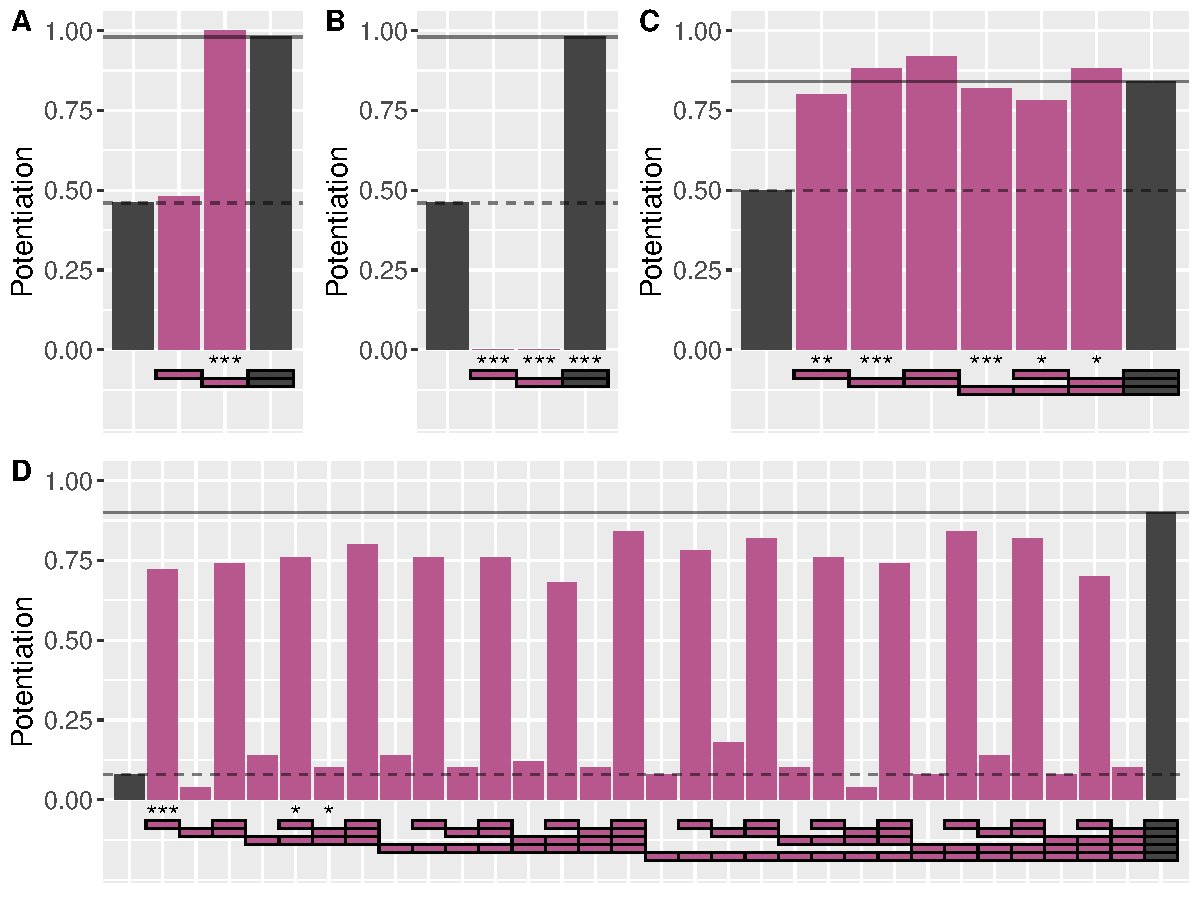
\includegraphics[width=0.9\textwidth]{04_learning_extension/media/mut_splits.pdf}
\end{center}
\caption{ 
Selected results from the mutation split experiment. 
For each subplot, the rightmost column shows the potentiation immediately after the largest potentiating step in that replicate (also shown via solid horizontal line), and the leftmost column shows the potentiation immediately before that step in the lineage (also shown via dashed horizontal line). 
This potentiating step involved $N$ mutations, where $N$ is 2 for subplots A and B, 3 for subplot C, and 5 for subplot D.
There are a total of $2^N$ bars in each subplot, representing the $2^N$ possible combinations of these mutations, as indicated by the small boxes below each bar.
The left bars show potentiation with none of the $N$ mutations presents, the right bars have all $N$ mutations present,
%These two steps are separated by $N$ mutations,
and the middle bars (purple) show the potentiation of every other possible combination of these mutations. 
Significance of each mutation combination in the logistic regression is shown under each column (* for $p \leq 0.05$, ** for $p \leq 0.01$, *** for $p \leq 0.001$). 
%Finally, the small boxes show the presence of individual mutations, with columns increasing in binary order.
In subplots A and D potentiation is driven by just one of the mutations; in B potentiation requires both mutations (which are individually lethal); and in C all three mutations are independently-potentiating. 
}\label{fig:mut_splits}
\end{figure}

For each of the learning lineages, we have identified the potentiating step; that is, the step in the phylogeny that conferred the largest increase in potentiation. 
Since Avida has a per-site rate for substitution mutations, and insertion and deletion mutations that can occur simultaneously, these lineage steps can consist of more than one mutation. 
Even so, 60\% of the potentiating steps (30 of 50) are comprised of only one mutation. 
Of the remaining 20 potentiating steps, 14 steps contained two mutations, three steps contained three mutations, one step contained four mutations, and two steps contained five mutations. 

Of course, the 30 potentiating steps that consisted of a single mutation must be driven by that particular mutation. 
For each of the other 20 potentiating steps (where multiple mutations co-occurred), we ran replay experiments to split the mutations and determined that not all were necessary to increase potentiation. 
Indeed, % of the 20 steps that consisted of more than one mutation, 
in 14 cases we identified exactly one mutation that significantly increased potentiation on its own. 
The two steps involving five-mutation are included here, as a single mutation explained the potentiation gain in both cases. 
Data from an example of potentiation being driven by one of two co-occurring mutations can be seen in Figure \ref{fig:mut_splits}A, and an example of one driving mutation out of five total mutations can be seen in Figure \ref{fig:mut_splits}D. 

As discussed above, other work has shown that single mutations can have a large impact on potentiation. 
This has been shown in colistin resistance in \textit{Pseudomonas aeruginosa} \citep{jochumsenEvolutionAntimicrobialPeptide2016a} and in the evolution of EQU in Avida \citep{covertiiiExperimentsRoleDeleterious2013}.
Thus we have instances where potentiation increases drastically with single mutations in both digital and natural organisms. 
% Conversely, while we see some evidence for the slow accumulation of potentiation (i.e, 50-step windows with significant potentiation gain but no individual mutations within the window that significantly increase potentiation), we have not found evidence of this dynamic in natural systems in the potentiation literature. 


\subsection{Mutation interactions influence potentiation}
% Mutation interactions influence potentiation
    % Of the 6 replicates that did not rely on one single mutation, at least four had interesting interactions among there mutations
    % Two had epistatic interactions -- the individual mutations were lethal, but together they were potentiating
    % One had two mutations additively accounting for the increase in potnetiation
    % One had three independent mutations, where each mutation would have increased potentiation, but the combination did nothing
    % The final two had no significant factors, and thus we cannot classify them


While we are able to confidently say that many replicates saw potentiation increase with a single mutation, we also observed instances where potentiation changes appeared to require interactions across multiple simultaneous mutations, or other unexpected interactions. %, including their interactions, can influence potentiation.
We identified one replicate where two mutations independently increased potentiation, and combined they accounted for the full step's potentiation gain. 
In one of the steps containing three mutations, all three mutations independently increased potentiation significantly, but the combination of mutations did not further increase potentiation (Figure \ref{fig:mut_splits}C). 
In two replicates we see strong sign epistasis; each step consisted of two mutations, and when analyzed independently these mutations proved to be lethal (and thus potentiation is 0), but when the mutations were combined the resulting mutants were not only viable, but potentiated (Figure \ref{fig:mut_splits}B). 
This is akin to the case study of EQU potentiation in \citep{covertiiiExperimentsRoleDeleterious2013}, where two deleterious mutations (one nearly lethal) combined to actualize EQU.
Finally, of the 50 replicates, two were found to have no significant mutation effects, and further replicates would be required to disentangle the effects of the mutations and their interactions.

%\subsection{Potentiating mutations are still undetectable as they occur in an evolving population}
%\subsection{Potentiating mutations are cryptic in evolving populations}
\subsection{No real-time hallmarks of potentiating mutations were evident in an evolving population}

\begin{figure}[h!]
\begin{center}
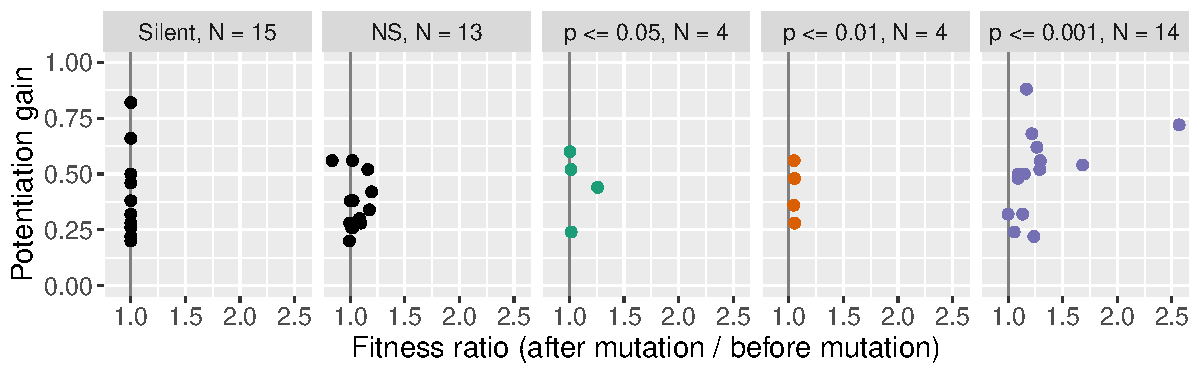
\includegraphics[width=0.9\textwidth]{04_learning_extension/media/fitness_diffs.pdf}
\end{center}
\caption{ 
The fitness effect and potentiation gain of the potentiating step of all 50 learning replicates. 
To calculate fitness, both the potentiation step and the step before it were evaluated on the same set of 100 random seeds. 
We ran a paired Wilcoxon rank-sum test for these two fitness groups for each replicate, and divided and colored the results based on these significance findings. 
Non-significant points are split into those that are truly silent mutations (i.e., zero change in fitness across all 100 trials) and those that are not (fitness values changed, but not significantly). 
The fitness ratio, used for the x-axis, is calculated as the average post-mutation fitness divided by the average pre-mutation fitness. 
The vertical line shows a fitness ratio of one, which indicates no change in the average effect. 
}\label{fig:fitness_diffs}
\end{figure}

As discussed in Chapter \ref{chap:learning_case_studies}, while we can retrospectively identify potentiating mutations, we have yet to find strong indicators of these mutations \textit{during evolution}.
Any such consistent indicators would be invaluable for problem solving with evolutionary computation or other forms of applied evolution. 

Our early hypothesis was that these potentiating mutations are likely to be deleterious, or at least neutral. 
Our reasoning was that if the mutations are beneficial, they would already be likely to be selected and thus they would already be factored into  %expect that their appearance would not drastically alter long-term 
evolutionary potential. 
Of the four case study lineages in Chapter \ref{chap:learning_case_studies}, we saw that one potentiating step was deleterious, two were neutral, and one was beneficial. 

Here, we have refined our methods to compare the potentiating step to the step before it, evaluating both genotypes on the same set of 100 random paths to conduct a pairwise comparison (Figure \ref{fig:fitness_diffs}). 
Using a paired Wilcoxon test, we find that in 28 of 50 lineages the potentiating step did not have a significant effect on realized fitness. 
Indeed, in 15 of these replicates, the two genotypes displayed \textit{exactly} the same behavior -- the mutations were truly silent, while in 13 changes to fitness occurred, but not enough to meaningfully change the distribution.
The truly neutral mutations may be modifying instructions that are executed but do not directly effect the phenotype, or they could be cryptic genetic variation occurring in unexpressed regions of the genotype (Chapter \ref{chap:consequences_of_plasticity}). 
Of the remaining 22 replicates with significant changes to fitness, we find that 21 significantly increase fitness, and only one mutation was significantly deleterious. 
Further, our one deleterious mutation was significant ($p < 0.001$) but not substantial, with less than a 1\% change in fitness. 

The fitness effects of the significantly beneficial mutations varied wildly,  with many conferring small impacts on fitness. 
Two mutations had a greater than 50\% increase in fitness, one of which had a fitness over 250\% of the pre-mutation fitness. 
Thus, we have strong evidence against our hypothesis that potentiating mutations are likely deleterious. 
We observe that potentiating mutations are often neutral or nearly-neutral, though they can also drastically increase fitness. 
%In a genetic space as complicated as Avida's, we now realize that even if a mutation is highly beneficial, there are likely other highly-beneficial mutations, even if they are few, and thus these beneficial mutations are not guaranteed to sweep and thus can affect potentiation.
In a genetic space as complicated as Avida's, even highly-beneficial mutations are not guaranteed to be found, let alone sweep.
Given the number of alternative possibilities, some of which may be highly advantageous themselves, even beneficial mutations can be highly potentiating.
Indeed, even if deleterious mutations would open up new pathways through the genotype space, the low probability of them gaining substantial numbers in the population may eliminate the possibility of them being potentiating.

One final hypothesis for identifying potentiation mutations \textit{as they occur} is to look for mutations that alter the overall behavioral phenotype. 
Of the 50 potentiating lineage steps that we analyzed, we found that 43 of 50 left the underlying behavioral phenotype unchanged. 
Of the seven that did change the phenotype, all were originally error correction behaviors. 
After the potentiating step, five then shifted to a mixed bet hedging strategy -- they still performed error correction on some paths but were capable of learning on others. 
One more replicate evolved learning \textit{with the potentiating step}, likely representing a low probability mutation that was actualized. 
The final behavior-changing mutation shifted the behavior from error correction to bet-hedged error correction. 
While this replicate might represent an interesting case -- the degradation of behavior -- the majority of potentiating mutations did not change the behavior and thus behavior changes are not a reliable indicator of potentiating mutations when they occur. 